\section{Анализ Neural Tangent Kernel}

\subsection{Введение}

Neural Tangent Kernel (NTK) представляет собой ядро, индуцированное нейронной сетью через градиенты выхода сети по её параметрам. В современной теории глубокого обучения NTK играет важную роль, поскольку позволяет описывать обучение нейронной сети в функциональном пространстве, а не только в пространстве параметров. Это особенно важно в режиме большой ширины, когда динамика градиентного спуска приобретает почти линейный характер и становится близкой к обучению ядрового метода.

Ключевая идея состоит в том, что при достаточно большой ширине скрытых слоёв случайно инициализированная сеть ведёт себя почти как линейная модель относительно параметров в окрестности точки инициализации. В этом пределе NTK стремится к детерминированному ядру, а обучение сети по градиентному спуску оказывается эквивалентным kernel regression с данным ядром. Поэтому NTK служит мостом между теорией глубоких сетей, гауссовскими процессами и классическими ядровыми методами.

\subsection{Математическое обоснование}

\subsubsection{Определение NTK}

Пусть нейронная сеть задаёт скалярную функцию
\begin{equation}
    f(x,\theta): \mathbb{R}^d \to \mathbb{R},
\end{equation}
где $x$ --- вход, а $\theta \in \mathbb{R}^p$ --- вектор параметров сети. Для двух входов $x$ и $x'$ Neural Tangent Kernel определяется как скалярное произведение градиентов выхода сети по параметрам:
\begin{equation}
    K(x,x';\theta)=\nabla_{\theta} f(x,\theta)^{\top}\nabla_{\theta} f(x',\theta).
    \label{eq:ntk_def}
\end{equation}

Если рассматривать набор точек $X=\{x_i\}_{i=1}^{n}$, то соответствующая матрица NTK имеет вид
\begin{equation}
    \Theta_{ij}(\theta)=K(x_i,x_j;\theta)=\nabla_{\theta} f(x_i,\theta)^{\top}\nabla_{\theta} f(x_j,\theta).
    \label{eq:ntk_matrix}
\end{equation}

Иначе говоря, NTK измеряет сходство двух входов не в исходном пространстве признаков, а в пространстве чувствительности модели к своим параметрам.

\subsubsection{Переход к линейной динамике обучения}

Рассмотрим обучение по функции потерь среднеквадратичного отклонения
\begin{equation}
    \mathcal{L}(\theta)=\frac{1}{2}\sum_{i=1}^{n}\bigl(f(x_i,\theta)-y_i\bigr)^2.
\end{equation}
В режиме непрерывного времени градиентный спуск записывается как gradient flow:
\begin{equation}
    \frac{d\theta}{dt}=-\nabla_{\theta}\mathcal{L}(\theta)
    =-\sum_{j=1}^{n}\bigl(f(x_j,\theta)-y_j\bigr)\nabla_{\theta}f(x_j,\theta).
    \label{eq:gradient_flow_theta}
\end{equation}

Обозначим через
\begin{equation}
    u_i(t)=f(x_i,\theta(t)), \qquad u(t)=\bigl(u_1(t),\dots,u_n(t)\bigr)^{\top}.
\end{equation}
Тогда по правилу цепочки
\begin{equation}
    \frac{du_i}{dt}
    =\nabla_{\theta}f(x_i,\theta)^{\top}\frac{d\theta}{dt}.
\end{equation}
Подставляя \eqref{eq:gradient_flow_theta}, получаем
\begin{equation}
    \frac{du_i}{dt}
    =-\sum_{j=1}^{n}\Theta_{ij}(\theta)\bigl(u_j(t)-y_j\bigr).
\end{equation}
В матричной форме это даёт
\begin{equation}
    \frac{du}{dt}=-\Theta(\theta(t))\bigl(u(t)-y\bigr).
    \label{eq:functional_dynamics}
\end{equation}

Формула \eqref{eq:functional_dynamics} показывает, что именно матрица NTK определяет скорость уменьшения ошибки по различным направлениям в пространстве функций. Если в ходе обучения ядро меняется мало, то можно считать
\begin{equation}
    \Theta(\theta(t))\approx \Theta(\theta_0)=\Theta_0,
\end{equation}
и тогда динамика становится линейной:
\begin{equation}
    \frac{du}{dt}=-\Theta_0\bigl(u(t)-y\bigr).
\end{equation}
Решение этой системы имеет вид
\begin{equation}
    u(t)-y=\exp(-\Theta_0 t)\bigl(u(0)-y\bigr).
    \label{eq:matrix_exp_solution}
\end{equation}

Таким образом, компоненты ошибки, соответствующие большим собственным значениям NTK, затухают быстрее, тогда как направления, связанные с малыми собственными значениями, обучаются медленнее.

\subsubsection{Связь с kernel regression}

Пусть обучение ведётся до интерполяции обучающих данных, а NTK остаётся практически постоянным. Тогда предельное решение для нового входа $x$ можно записать в форме ядровой регрессии:
\begin{equation}
    f_{\infty}(x)=f_0(x)+\Theta(x,X)\Theta(X,X)^{-1}\bigl(y-f_0(X)\bigr),
    \label{eq:kernel_regression_ntk}
\end{equation}
где $f_0$ --- функция, соответствующая инициализации, $\Theta(x,X)$ --- строка значений NTK между точкой $x$ и обучающим набором, а $\Theta(X,X)$ --- Gram-матрица NTK на обучающей выборке.

Следовательно, в \emph{lazy training regime} широкая нейронная сеть фактически обучается как ядровой метод, в котором ядро не задаётся заранее вручную, а индуцируется архитектурой и инициализацией сети.

\subsubsection{Почему NTK стабилизируется при большой ширине}

Для широких сетей вклад отдельных нейронов в суммарный выход мал, а сама сеть содержит большое количество независимых или слабо зависимых случайных компонентов. В результате, по закону больших чисел, матрица NTK при случайной инициализации концентрируется около детерминированного предела:
\begin{equation}
    \Theta(\theta_0) \xrightarrow[m\to\infty]{} \Theta_{\infty},
\end{equation}
где $m$ обозначает ширину скрытых слоёв. Более того, при подходящей параметризации изменения параметров в процессе обучения имеют порядок, недостаточный для существенного изменения ядра, поэтому
\begin{equation}
    \Theta(\theta(t)) \approx \Theta(\theta_0) \approx \Theta_{\infty}
\end{equation}
на конечном промежутке времени. Именно это и приводит к почти линейной динамике обучения.

\subsection{Интуитивная интерпретация}

Интуитивно NTK измеряет не просто близость входов $x$ и $x'$, а то, насколько похожим образом сеть будет изменять своё предсказание в этих двух точках при бесконечно малом изменении параметров. Если градиенты $\nabla_{\theta} f(x,\theta)$ и $\nabla_{\theta} f(x',\theta)$ направлены почти одинаково, то обновление параметров, уменьшающее ошибку в точке $x$, будет одновременно существенно влиять и на точку $x'$. Следовательно, соответствующее значение NTK будет большим.

С этой точки зрения NTK задаёт геометрию обобщения: он определяет, как локальное исправление ошибки переносится на другие объекты выборки. Поэтому NTK можно рассматривать как оператор распространения информации по данным. Если две точки имеют большой NTK, то сеть склонна обучать их совместно; если значение мало или близко к нулю, то их динамика обучения почти независима.

\subsection{Свойства NTK}

\subsubsection{Симметричность и положительная полуопределённость}

Из определения \eqref{eq:ntk_def} непосредственно следует симметричность:
\begin{equation}
    K(x,x';\theta)=K(x',x;\theta).
\end{equation}

Для любой конечной выборки $X=\{x_i\}_{i=1}^{n}$ матрица $\Theta(X,X)$ является положительно полуопределённой. Действительно, для любого вектора $c \in \mathbb{R}^n$ имеем
\begin{equation}
    c^{\top}\Theta c
    =\sum_{i,j=1}^{n}c_i c_j \nabla_{\theta}f(x_i,\theta)^{\top}\nabla_{\theta}f(x_j,\theta)
    =\left\|\sum_{i=1}^{n} c_i \nabla_{\theta}f(x_i,\theta)\right\|_2^2 \ge 0.
\end{equation}
Следовательно, собственные значения NTK в точной арифметике неотрицательны. Небольшие отрицательные значения на практике обычно связаны с численными погрешностями.

\subsubsection{Спектр собственных значений}

Пусть
\begin{equation}
    \Theta = Q \Lambda Q^{\top}, \qquad
    \Lambda=\mathrm{diag}(\lambda_1,\dots,\lambda_n), \qquad
    \lambda_1 \ge \lambda_2 \ge \dots \ge \lambda_n \ge 0.
\end{equation}
Тогда спектр $\{\lambda_i\}$ показывает, насколько много независимых направлений изменения функции реально доступно сети на рассматриваемой выборке. Быстрый спад спектра означает, что обучение в основном происходит в низкоразмерном подпространстве, тогда как медленный спад указывает на более богатую функциональную динамику.

Важными характеристиками являются:
\begin{equation}
    \mathrm{trace}(\Theta)=\sum_{i=1}^{n}\lambda_i,
\end{equation}
\begin{equation}
    \mathrm{rank}(\Theta)=\#\{i:\lambda_i>0\},
\end{equation}
а также effective rank, определяемый через энтропию нормированных собственных значений:
\begin{equation}
    p_i=\frac{\lambda_i}{\sum_j \lambda_j}, \qquad
    r_{\mathrm{eff}}=\exp\left(-\sum_i p_i \log p_i\right).
\end{equation}

\subsubsection{Condition number}

Для положительных собственных значений condition number определяется как
\begin{equation}
    \kappa(\Theta)=\frac{\lambda_{\max}}{\lambda_{\min}^{+}},
\end{equation}
где $\lambda_{\min}^{+}$ --- наименьшее положительное собственное значение. Если $\kappa(\Theta)$ велико, то задача плохо обусловлена: одни компоненты ошибки убывают очень быстро, а другие --- крайне медленно. Это соответствует жёсткой динамике обучения и повышенной чувствительности к шуму и численным ошибкам.

\subsubsection{Что означает ``хорошее'' и ``плохое'' NTK}

С практической точки зрения ``хорошее'' NTK характеризуется следующими свойствами:
\begin{enumerate}
    \item матрица имеет отчётливую информативную структуру, отражающую геометрию данных;
    \item спектр не вырождается слишком быстро;
    \item малые собственные значения не слишком близки к нулю;
    \item condition number остаётся умеренным.
\end{enumerate}

``Плохое'' NTK, напротив, может быть почти вырожденным, иметь чрезвычайно большой condition number или демонстрировать слабую связь между объектами, которые по смыслу должны обучаться совместно. В этом случае сеть может плохо переносить информацию между близкими по задаче точками и медленно обучаться в ряде направлений.

\subsection{Связь с Gaussian Process и режимом lazy training}

В пределе бесконечной ширины случайно инициализированная нейронная сеть при фиксированной архитектуре индуцирует Gaussian Process (точнее, распределение её выходов на конечном наборе входов стремится к гауссовскому). Однако Gaussian Process описывает \emph{априорное} распределение функций до обучения, тогда как NTK определяет \emph{динамику обучения} в функциональном пространстве. Поэтому GP и NTK отражают два разных аспекта одной и той же широкой сети: GP характеризует случайную функцию на инициализации, а NTK --- то, как эта функция будет изменяться под действием градиентного спуска.

Режим lazy training соответствует ситуации, когда параметры сети смещаются относительно мало, а сама функция хорошо аппроксимируется первым членом разложения Тейлора:
\begin{equation}
    f(x,\theta)\approx f(x,\theta_0)+\nabla_{\theta}f(x,\theta_0)^{\top}(\theta-\theta_0).
\end{equation}
В этом режиме обучение широкой нейронной сети практически эквивалентно обучению линейной модели в пространстве случайных признаков, заданных градиентами по параметрам.

\subsection{Практический пример: вычисление NTK для MLP}

Для практической демонстрации рассмотрим полносвязную сеть (MLP) с двумя скрытыми слоями и нелинейностью $\tanh$. На конечной выборке $\{x_i\}_{i=1}^{n}$ эмпирический NTK вычисляется следующим образом:
\begin{enumerate}
    \item для каждого входа $x_i$ вычисляется градиент $\nabla_{\theta} f(x_i,\theta)$;
    \item градиенты векторизуются и собираются в матрицу Якоби $J \in \mathbb{R}^{n \times p}$;
    \item матрица NTK строится как
    \begin{equation}
        \Theta = J J^{\top}.
    \end{equation}
\end{enumerate}

Ниже приведён компактный пример на Python/PyTorch, вычисляющий NTK на toy-задаче регрессии и сравнивающий ядро до и после обучения:

\begin{verbatim}
import torch
import torch.nn as nn
import matplotlib.pyplot as plt

class MLP(nn.Module):
    def __init__(self, width=128):
        super().__init__()
        self.net = nn.Sequential(
            nn.Linear(1, width), nn.Tanh(),
            nn.Linear(width, width), nn.Tanh(),
            nn.Linear(width, 1)
        )
    def forward(self, x):
        return self.net(x)

def empirical_ntk(model, x):
    params = [p for p in model.parameters() if p.requires_grad]
    grad_rows = []
    for i in range(x.shape[0]):
        model.zero_grad(set_to_none=True)
        y = model(x[i:i+1]).squeeze()
        grads = torch.autograd.grad(y, params)
        grad_rows.append(torch.cat([g.reshape(-1) for g in grads]).detach())
    J = torch.stack(grad_rows, dim=0)
    K = J @ J.T
    return 0.5 * (K + K.T)

x = torch.linspace(-2.0, 2.0, 32).unsqueeze(1)
y = torch.sin(3.0 * x) + 0.2 * x
model = MLP(width=128)
K_before = empirical_ntk(model, x)

opt = torch.optim.Adam(model.parameters(), lr=1e-3)
loss_fn = nn.MSELoss()
for _ in range(1500):
    opt.zero_grad(set_to_none=True)
    loss = loss_fn(model(x), y)
    loss.backward()
    opt.step()

K_after = empirical_ntk(model, x)
eig_before = torch.linalg.eigvalsh(K_before).flip(0)
eig_after = torch.linalg.eigvalsh(K_after).flip(0)
\end{verbatim}

Полная воспроизводимая версия скрипта, строящая графики и сохраняющая метрики, находится в файле \texttt{scripts/ntk\_pytorch\_demo.py}.

\subsection{Визуализации и анализ результатов}

\begin{figure}[ht!]
    \centering
    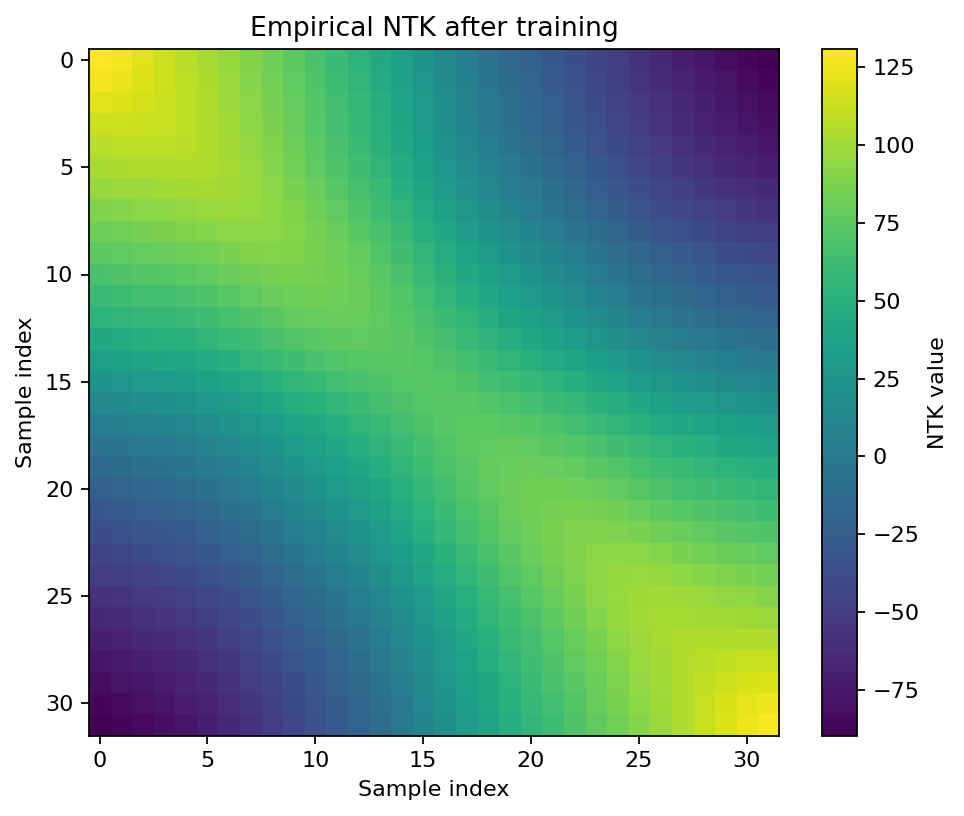
\includegraphics[width=0.72\textwidth]{../ntk_report_assets/ntk_heatmap_after.png}
    \caption{Эмпирическая матрица NTK после обучения MLP на toy-задаче одномерной регрессии. Яркая диагональ отражает сильную чувствительность предсказания в каждой точке к собственным градиентным направлениям, а выраженная вне диагональная структура показывает, что близкие входы оказываются связанными и обучаются не независимо, а согласованно.}
    \label{fig:ntk_heatmap_after}
\end{figure}

На \cref{fig:ntk_heatmap_after} видно, что NTK имеет не случайную, а упорядоченную структуру: элементы матрицы меняются плавно вдоль строк и столбцов. Это означает, что сеть переносит информацию локально по входному пространству. Для одномерных данных такая картина соответствует интуитивному ожиданию: соседние точки имеют схожие градиенты по параметрам, поэтому обновление сети в одной точке влияет на соседние.

\begin{figure}[ht!]
    \centering
    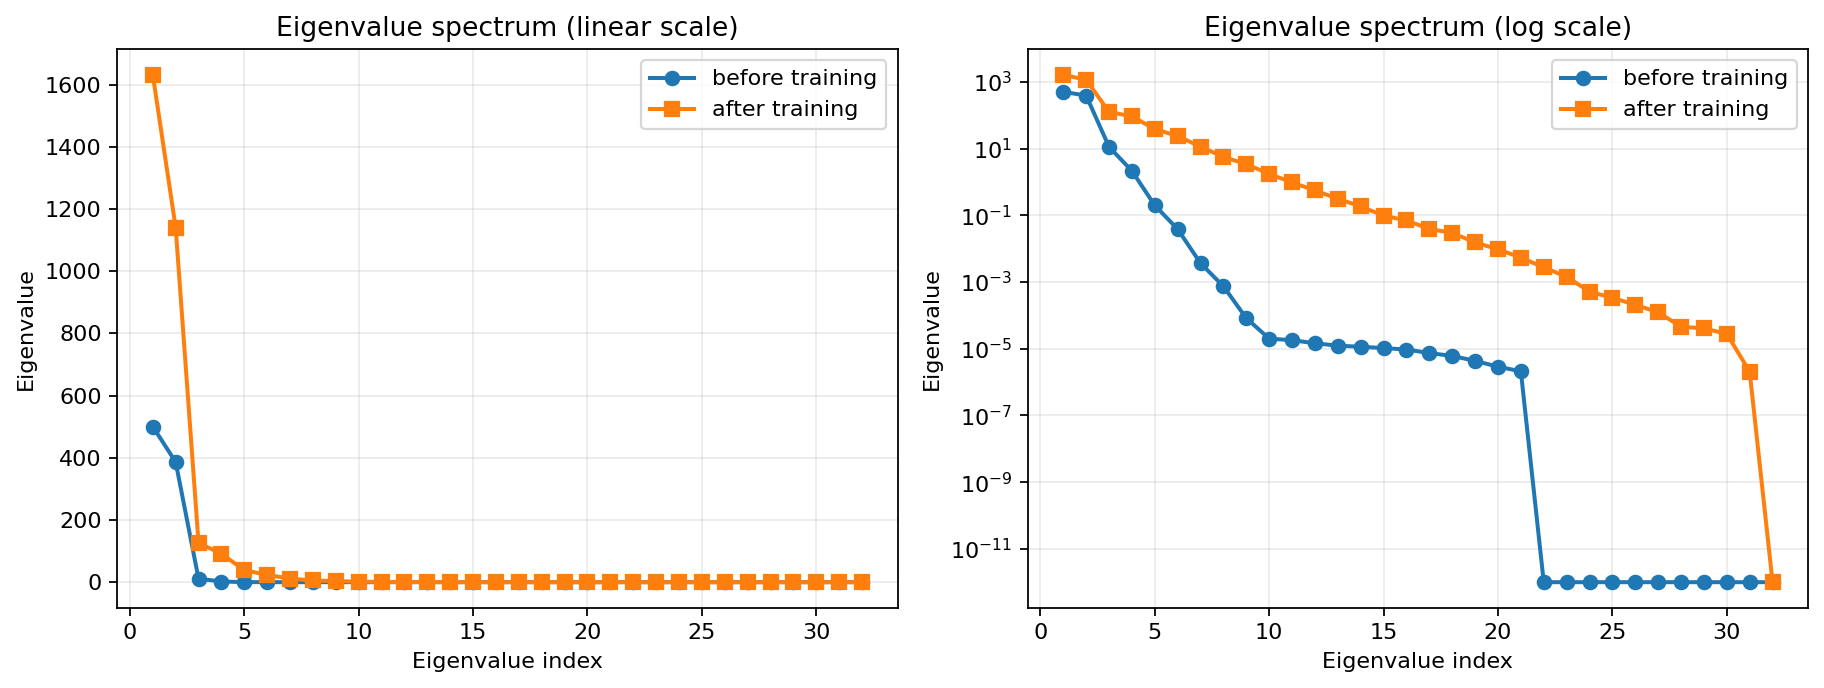
\includegraphics[width=\textwidth]{../ntk_report_assets/ntk_eigenspectrum_before_after.png}
    \caption{Спектр собственных значений NTK до и после обучения. Левая панель показывает спектр в линейном масштабе, правая --- в логарифмическом. После обучения доминирующие собственные значения возрастают, а сам спектр становится более протяжённым, что указывает на увеличение числа направлений в функциональном пространстве, по которым сеть активно адаптируется к данным.}
    \label{fig:ntk_spectrum}
\end{figure}

Из \cref{fig:ntk_spectrum} следует, что после обучения ведущие собственные значения увеличиваются, а спектр спадает медленнее. Это означает, что сеть усиливает чувствительность к нескольким главным направлениям данных и одновременно начинает использовать большее число мод обучения. Если же спектр спадает чрезвычайно быстро, это обычно указывает на близость ядра к низкоранговому и на ограниченную функциональную выразительность на рассматриваемой выборке.

\begin{figure}[ht!]
    \centering
    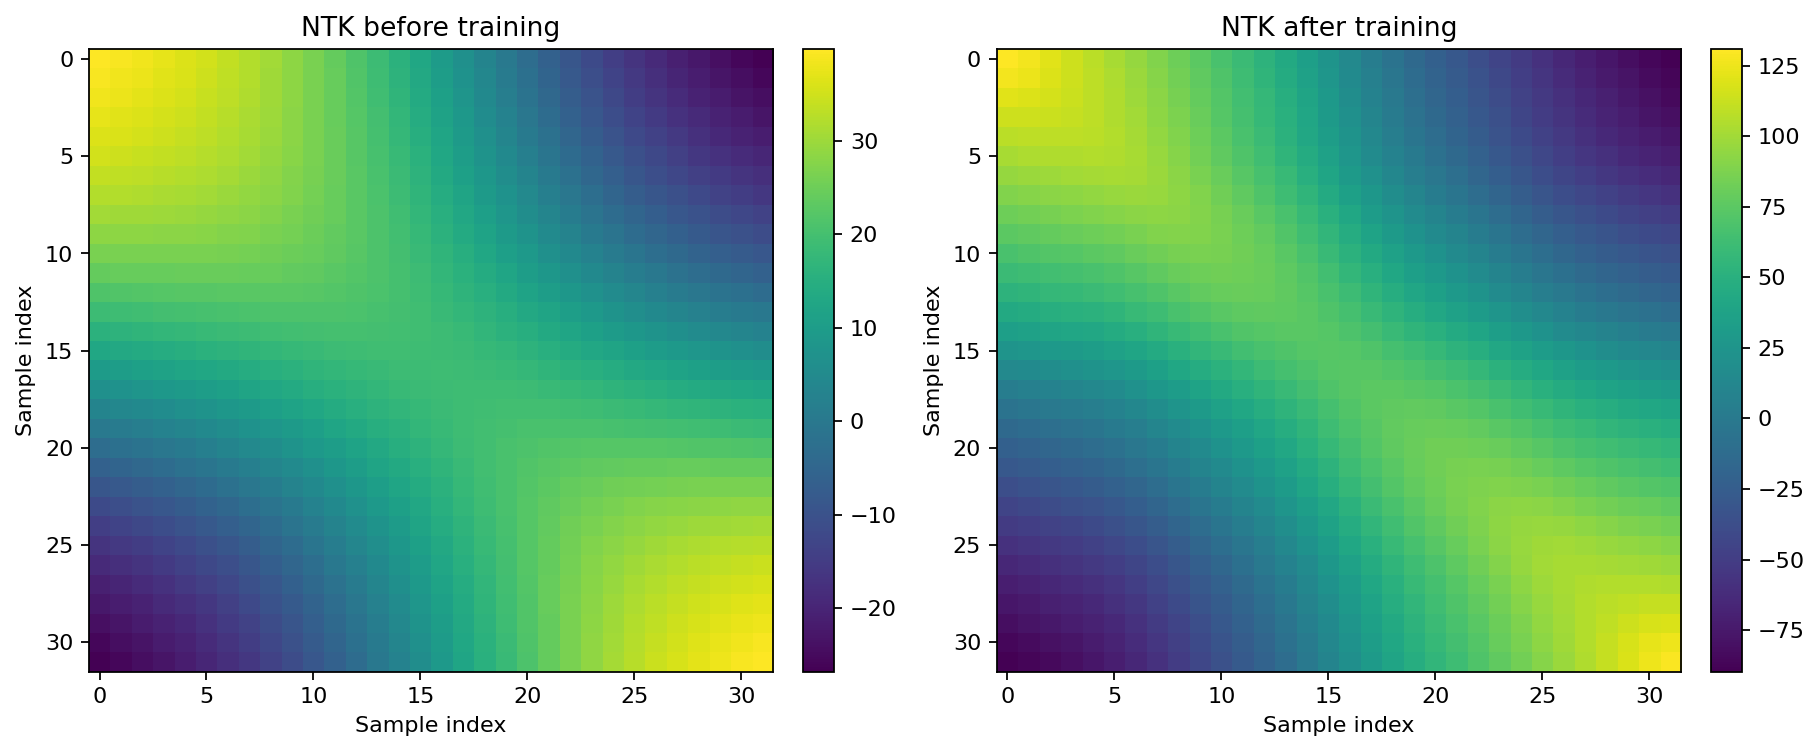
\includegraphics[width=\textwidth]{../ntk_report_assets/ntk_heatmaps_before_after.png}
    \caption{Сравнение матриц NTK до и после обучения. До обучения ядро определяется в основном архитектурой и случайной инициализацией; после обучения структура NTK становится более контрастной, что отражает перераспределение чувствительности модели в соответствии с геометрией данных и целевой функцией.}
    \label{fig:ntk_compare}
\end{figure}

\Cref{fig:ntk_compare} показывает, что даже если глобальная структура ядра сохраняется, обучение заметно изменяет масштаб и локальную неоднородность значений NTK. Это согласуется с тем, что для конечной ширины сеть не обязана полностью оставаться в режиме постоянного ядра: на практике NTK может эволюционировать, хотя для очень широких сетей и малых перемещений параметров эта эволюция обычно слабее.

\subsection{Интерпретация результатов}

Heatmap матрицы NTK позволяет выявлять структуру данных. Если на карте заметны блочные области, это свидетельствует о существовании групп объектов, которые сеть воспринимает как близкие с точки зрения градиентной геометрии. Для упорядоченных одномерных или временных данных нередко наблюдается полосатая или ленточная структура, указывающая на локальное распространение информации.

Спектр собственных значений показывает, какие функциональные моды осваиваются быстрее всего. Большие собственные значения соответствуют направлениям, по которым ошибка убывает быстро; малые --- направлениям, требующим существенно большего времени обучения. Поэтому спектр NTK непосредственно связан с динамикой оптимизации. Кроме того, effective rank служит удобной характеристикой ``эффективной размерности'' функционального пространства, используемого сетью на данной выборке.

Связь NTK с обобщающей способностью проявляется через согласование спектра ядра со структурой целевой функции. Если полезный сигнал хорошо проецируется на ведущие собственные векторы ядра, сеть обучается быстро и, как правило, демонстрирует более устойчивое поведение вне обучающей выборки. Если же значимая часть целевой функции лежит в направлениях, отвечающих очень малым собственным значениям, обучение будет медленным и чувствительным к шуму. Следовательно, хорошее обобщение в NTK-подходе связано не только с шириной сети или размером выборки, но и с тем, насколько индуктивное смещение архитектуры согласуется со структурой задачи.

\subsection{Выводы по разделу}

NTK даёт строгий математический язык для описания обучения нейронных сетей в терминах ядровых методов. Он определяется через градиенты выхода по параметрам, задаёт линейную динамику обучения в режиме почти постоянного ядра и связывает широкие нейронные сети с kernel regression. Анализ спектра NTK, его ранга, effective rank и condition number позволяет судить о качестве индуцированного ядра, о скорости обучения различных мод и о том, насколько архитектура сети согласована со структурой данных. В этом смысле NTK является не только теоретическим объектом, но и практическим инструментом анализа динамики и обобщающей способности нейросетевых моделей.
